\documentclass{ctuthesis}
\usepackage[ruled,vlined,linesnumbered]{algorithm2e}

\ctusetup{
    xdoctype = B,
    xfaculty = F3,
    mainlanguage = english,
    titlelanguage = english,
    title-english = {Expedition scheduling in an automated warehouse},
    title-czech = {Rozvrhování vyskladňování z automatizovaného skladu},
    specification-file = {zav_prace.pdf},
    front-specification = true,
    department-english = {Department of Computer Science},
    author = {Jan Kalina},
    supervisor = {Ing. Martin Schaefer},
    supervisor-address = {Unknown,\\ Zářivá 232,\\
      12000 Praha 2},
      day = 13,
    month = 5,
    year = 2019,
    keywords-english = {scheduling, automated warehouse, optimization, simulation},
}

\ctuprocess

\begin{thanks}

TBD
\end{thanks}

\begin{declaration}

Prohlašuji, že jsem předloženou práci vypracoval
samostatně a že jsem uvedl veškeré použité informační zdroje v souladu
s Metodickým pokynem o dodržování etických principů při přípravě vysokoškolských
závěrečných prací.
\medskip


V Praze, \ctufield{day}.~\monthinlanguage{second}~\ctufield{year}

\end{declaration}
\begin{abstract-english}
This thesis deals with the optimization problem of expedition scheduling in an automated warehouse with a given set of parameters, requirements and set of items to dispatch in a day. Relevant scheduling problems and their solutions are discussed. Optimization method and objectives are then proposed for the given type of an automated warehouse. The proposed method is implemented in the provided simulation tool and evaluated based on its performance in the simulation.

\end{abstract-english}



\begin{abstract-czech}
test \ldots
\end{abstract-czech} 

\begin{document}

\maketitle

\chapter{Introduction}

Scheduling is a well studied and practical topic. It is widely used in manufacturing facilities, warehouses, which are discussed in this thesis, and many other industries where proper scheduling can play a great role in their success. Despite its importance and years of research, scheduling is quite a challenging problem, especially when it comes to real-world problems where finding an optimal schedule is usually nearly impossible due to its high computational complexity. 

Since the beginning of research in scheduling, many methods and approaches were developed for finding schedules close to optimal schedule in a reasonable time, but what is a good or optimal schedule? Determining the objective of a schedule is a problem on its own. The usual objective of scheduling is to minimize the makespan, which is the duration of a schedule. This objective alone is usually not sufficient because it does not consider the stochastic nature of real-world, where random events can change the schedule for the worse. In that case, the most valuable schedule might be the one where these random events change a schedule the least and makespan is still small. Another reason why makespan or other simple objectives that are often mentioned in literature might not be sufficient is that some facilities may demand complex customized requirements tailored just for them. For example, in case of an automated warehouse, it may be crucial to not only finish expedition in required time but to also expedite items in the required order. 

In this thesis, general methods for solving scheduling problems relevant to scheduling a daily expedition of the given automated warehouse configuration are discussed. Then, method and an objective of a schedule for the given automated warehouse and scenario is proposed. Finally, proposed method is implemented and evaluated based on results from the provided simulation tool. 

\section{The automated warehouse}
\label{sec:wh}
There are many different types of automated warehouses with very different requirements, structures, and functionality. The problem of scheduling an expedition can be very different based on the structure and the type of an automated warehouse. The basic structure and functionality of an automated warehouse based on a real-world problem were provided for this thesis and can be described as follows.

\subsection{Description}
\label{subsec:Description}
The automated warehouse is part of a factory. This factory stores products to the automated warehouse from which they are at some point expedited. Firstly, we describe production together with the automated warehouse and secondly we describe the expedition process.

\subsubsection{Production and the automated warehouse}

Factory produces up to 20 thousand items throughout a whole day. Items come in hundreds of different types, which may differ in size, material or in other properties, which are not important for this thesis. Since the warehouse is automated, items must have suitable weight and size to be handled by a stacker crane and to be stored in high-bay racks. The example of such items are tires or pallets of different sodas. Produced items are directly put one-by-one on the conveyor leading to the warehouse, where an item is pushed off the conveyor to the production buffer of one of the aisles.

The automated warehouse has given number of aisles. Each aisle has high-bay racks on both sides and is connected to two conveyors at the beginning of it. The first conveyor is moving items from an aisle to one of the expedition ramps, and the second is bringing in items from production. Each aisle has a single stacker crane operating on it.

Stacker cranes operate automatically and can either store an item from production if it is available or execute scheduled unloadings. 

//detailed stacker crane
If stacker crane is requested to unload an item, it moves to the position of an item, grabs it and moves to the beginning of an aisle, where it puts the item on the conveyor leading to a expedition ramp. In case of an item arriving from production to an aisle's production buffer. Stacker crane should retrieve this item from the production buffer and store in a free position in the aisle. If any production buffer overflows, production would have to be stopped, for that reason, stacker cranes prioritize storing of an item over unloading. It means that as soon as a stacker crane finishes an operation in progress, it stores an item from production even if it means delaying scheduled unloadings.

\subsubsection{Daily expedition}
Expedition is spanned over a part of one day. It is set when the working hours start and end. During the expedition, a truck can arrive at an expedition ramp at a scheduled time. Only one truck and be loaded at a time at each expedition ramp. There is also reserved time after which the next truck can arrive. Every truck requests a certain number of items of different types and order of these types in which they should be loaded into the truck for practical reasons. Which specific items will be expedited is known in advance and is expected that these items are distributed uniformly across all aisles. 

Before each item reaches an expedition ramp, it needs to be processed by a scanner, which is located at the end of the conveyor. 
//detailed scanner *reread
The order in which items they are processed by a scanner corresponds to order at which they are loaded into a truck. Scanners accept an item periodically. Since the scanner is processing items in the given interval, there has to be space between items on conveyor based on the speed of the conveyor and the duration of the interval. If many items arrive too soon after each other, they pile up and may cause the conveyor to stop, which should never happen. To prevent stopping of a conveyor, there is a small buffer. Scanner also accepts an item as soon as possible. The number of items that pile up in the buffer during a daily expedition will be one of the measurements of robustness to delays.

We also simplify our problem and assume that workers at the loading ramp can always pick up an item coming from the scanner. That means that scanners then create bottlenecks for each expedition ramp where throughput is limited by the frequency at which scanner can process items.


On top of all these specifications, it is expected that the expedition should not last longer than the working hours, but it also should not end too soon. Additionally, the duration of a truck expedition should not take too much time. These parameters and importance of these requests is something that client should specify and it has to be considered during a construction of a schedule.

\subsubsection{Available information}

Several basic parameters were provided for the given automated warehouse. These parameters include horizontal and vertical speeds and accelerations of stacker cranes, dimensions of a warehouse, speed and length of conveyors, duration of scanning an item, duration of grabbing an item from a conveyor, duration of putting an item on a conveyor and exact location of each item stored in the warehouse. For the expedition, we know count, types, and order at which items should be loaded for each truck. 


\begin{figure}
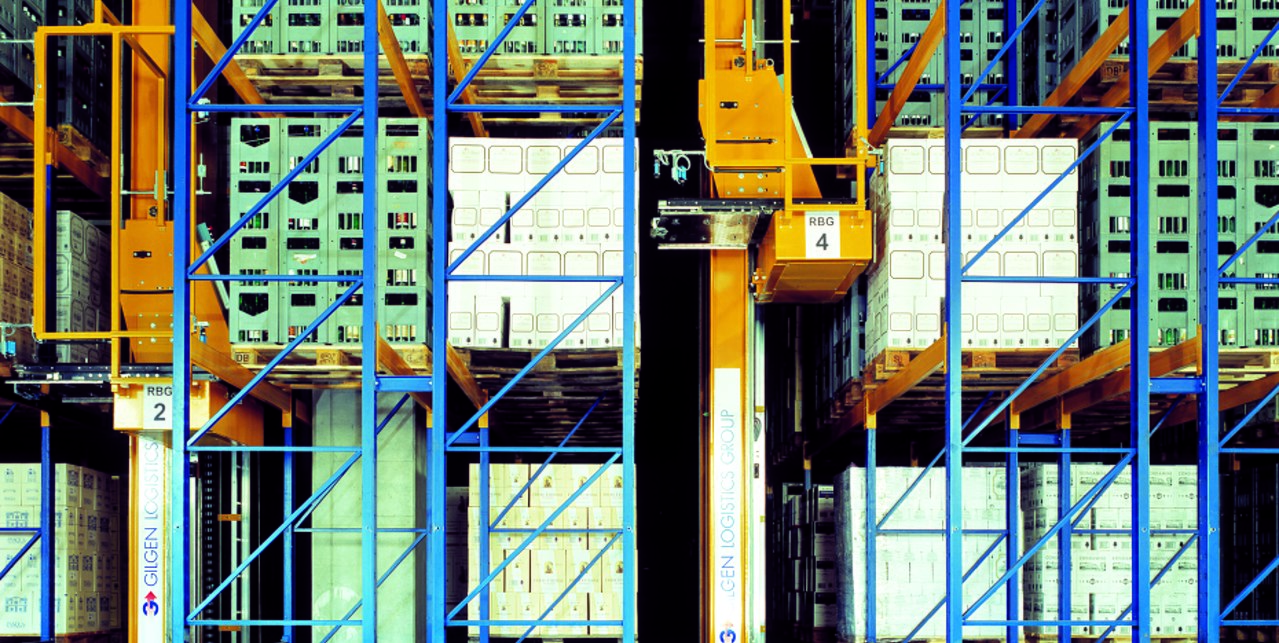
\includegraphics[width=0.8\linewidth]{highbaywarehouse.jpg}
\caption{Example of an automated warehouse with stacker cranes. \cite{warehousepic}}
\label{fig:foobar}
\end{figure}

\section{Goals and motivation}

The goal of this thesis is to create a schedule in reasonable time by assigning trucks planned for a day to expedition ramps, determining their order, determining order at which items will be expedited and finally determine specific time at which stacker cranes should start unloading each item. Since there is no information about item production, we cannot incorporate production handling in our schedule, but knowing that production handling can delay unloading of an item, we can try to minimize effect that production handling has on the schedule. How much production handling affects the schedule and if or how much are some of the requirements from Section \ref{sec:wh}, like preventing a buffer from filling up, violated sets how good the schedule is. To properly evaluate the schedule, it has to be integrated to provided simulation tool so that the created schedule can be observed in action and evaluated based on it. With a combination of the schedule and the simulation tool, we are also able to get data about the capabilities of the warehouse itself, which is valuable information when designing an automated warehouse. Integration of the scheduler to the simulation tool also enriches the simulation tool and can be used in future projects.

\section{Structure of this thesis}



\chapter{Problem statement}

\section{Notation and terminology}
in progress\\
\noindent \textbf{Job} ($job_i$) A $job_i$ represents an item $i$ to be expedited. Since expedition items are known in advance $job_i$ is already associated with one of the stacker cranes. 

\noindent \textbf{Machine} ($m_i$) A $m_i$ represents a stacker crane or a scanner. 

\noindent \textbf{Machine processing time} ($p_i$) Time which machine associated with $job_i$ needs to process $job_i$. In other words, the time needed to unload an item $i$ from its location to conveyor. This action consists of a trip from a conveyor to the item $i$, grabbing the item, trip back to the conveyor and putting the item on it. Values of $p_i$ are calculated from speeds, accelerations, and dimensions of the warehouse, but if production handling is taken into consideration, these values can become quite inaccurate since stacker crane may not always be at the same spot at the start of a job processing. Processing time is never zero.


\noindent \textbf{Scanning interval} ($s$) Processing time of a scanner. It is equal for every job.

\noindent \textbf{Traverse duration} ($t_i$)

\noindent \textbf{Completion time} ($c_i$)

\noindent \textbf{Assigned ramp} ($r_i$)

\noindent \textbf{Set of ramp ids} ($R$)

\noindent \textbf{Completion time of a truck} ($ct_i$)

\noindent \textbf{Start time} ($s_i$)

\noindent \textbf{Stacker crane completion time} ($scc_i$)

\noindent \textbf{Stacker crane start time} ($scs_i$)

\noindent \textbf{Position in expedition} ($pos_i$)

\noindent \textbf{Makespan}

\noindent \textbf{Reserve}

\noindent \textbf{Average flow time}

\noindent \textbf{Total flow time}

\noindent \textbf{TBD - expedition list, ... Add when needed} ($something_i$)


\section{Scheduling problem}
 
 The problem of expedition scheduling in the automated warehouse can be separated into two problems, trucks allocation and item dispatching. The first problem of truck allocation is dealing with assignment of ramps to trucks.
 
 The second problem, item dispatching, occurs after the truck allocation, and it deals with determining which items should meet which requests from trucks and the assignment of completion times of item unloading since machines are predetermined (see Section \ref{sec:wh}).
 
Both of these problems are described as machine models in following sections, which are used in scheduling literature (See \cite{pinedo} or \cite{bucker} for overview of machine models). More formal formulations for both of these problems are included.
 
 \subsection{Trucks allocation}
 \label{subsec:truckallocation}
This problem can be formulated as a parallel machine model.
 
 There are $r$ ramps in parallel and $t$ trucks planned for a day. Ramps can be interpreted as machines in parallel and jobs as the whole expedition of each truck. Since each ramp includes only one scanner, which acts as a bottleneck in the warehouse, the objective of this problem is to distribute expedition among ramps uniformly to utilize these ramps. In other words, workers at each expedition ramp should ideally work the same hours and do the same amount of work.
 
 The problem can be formulated as assignment problem as follows:
 
 \begin{equation}\label{eq:to}
\begin{aligned}
&\text{minimize}
&&\max(y_0, \ldots, y_r)
\end{aligned}
\end{equation}
\text{subject to}\\
\begin{equation} \label{eq:ta1}
\begin{aligned}
    & \sum_{i=0}^{n} x_{ij} = 1 && \text{for } j=0, \ldots, r\\
\end{aligned}
\end{equation}
\begin{equation} \label{eq:ta2}
\begin{aligned}
    & \sum_{i=0}^{t} {d_i} \cdot x_{ij} = y_j && \text{for } j=0, \ldots, r
\end{aligned}
\end{equation}
  
Where $x_{ij}$ is a binary decision variable, which detonates the $i$th truck is scheduled on $j$th expedition ramp. By satisfying Equation \ref{eq:ta1} it is ensured that every truck is assigned to only one ramp. Equation \ref{eq:ta2} sets variable $y_i$ to duration of expedition on the expedition ramp $i$. By minimizing Function \ref{eq:to} we minimize makespan, which leads the uniform utilization of machines \cite{pinedo}.
 
\subsection{Item dispatching}
\label{itemdispatching}
The problem of assigning completion times to jobs in the automated warehouse can be formulated as a special case of 2-stage flexible flow shop (FF2) with blocking or flexible flow line (FFL) with two stages as follows (See \cite{pinedo} for more information about these models):

There are two work stations connected in series. The first work stations consist of $m$ machines (stacker cranes) in parallel and the second work station consists of $r$ machines (scanners) also in parallel. Every job $job_i$ needs to be processed on its predetermined machine and processing of $job_i$ takes $p_i$ seconds. After job $job_i$ is processed, it travels $t_i$ seconds to get to a scanner where it needs to be processed too. Processing time $s$ of every scanner is the same. Jobs cannot wait between work stations. That alone is referred to as FFL.

For convenience we formulate this problem as constraint satisfaction problem as follows:

\textbf{Variables:}
\begin{align}
    &V = \{c_{0}, c_{1}, \ldots, c_{n},r_0, \ldots, r_m, pos_0, \ldots, pos_n\}
\end{align}
\textbf{Domains:}
\begin{align}
&c_{i} \in C_i = \{start, ..., end\} && \text{for } i=0,\ldots,n\\
&r_{i} \in R && \text{for } i=0,\ldots,n\\
&pos_i \in P_i
\end{align}
\textbf{Constraints:}
 \begin{align}
& pos_i < pos_j \iff c_i < c_j && \text{for } i=0,\ldots,n\\ \label{eq:idcons2}
& m_i = m_j \implies scc_i \leq scs_j \lor scc_j \leq scs_i && \text{for } i,j=0,\ldots,n\\ \label{eq:idcons1}
& r_i = r_j \implies c_i  + \theta_i \leq s_j \lor c_j + \theta_j \leq s_i && \text{for } i,j=0,\ldots,n\\ \label{eq:idcons4}
\end{align}

Where constraint \ref{eq:idcons2} ensures that a variable $pos_i$ represent an order at which an item $i$ is loaded. Constraints \ref{eq:idcons1} and \ref{eq:idcons4} secures that stacker cranes and scanners can process only one item at a time.
  
Alternatively, we can formulate this problem (with single expedition ramp) as a linear program, as follows:\\
\textbf{Decision variables}

\begin{itemize}
\item $x_{ij}$: 1 if $job_i$ expedited immediately after $job_j$, 0 otherwise
\item$c_i$: completion time of $job_i$ on the second stage
\item$idle_i$: idle time followed after $job_i$ on the second stage
\item$y_i$: order number of $job_i$ on the second stage
\item$scc_i$: start time of $job_i$ on the first stage 
\end{itemize}
\textbf{Data}
\begin{itemize}
\item$p_i$: processing time of $job_i$ on the first stage
\item$E_i$: set of allowed order numbers on the second stage for $job_i$
\item$I_i$: set of indexes of jobs scheduled on machine $i$ on the first stage
\item$M$: represents a large number
\item$start$: time at which work hours start
\item$end$: time at which work hours end
\end{itemize}

\begin{equation}
\begin{aligned}
&\text{minimize}
&&f(\ldots)
\end{aligned}
\end{equation}
\begin{equation}
\begin{aligned}
\text{subject to}\\
& \sum_{i=0}^{n} x_{ij} = 1 &&\\
& c_{i} - c_{j} + M(1 - x_{ij}) \geq s + idle_{i} && \text{for}\; i,j = 1, \ldots, n\\
& c_{i} - scc_{i0} = p_{i} + t_i + s + idle_i && \text{for}\; i = 1, \ldots, n\\
& scc_{i} + p_i < scc_j + M(1 - x_{ij}) && k = 0,\ldots,n, i,j \in I_k\\
& y_{i} - y_{j} < c_i - c_j + M(1 - x_{ij}) && \text{for}\; i,j = 1, \ldots, n\\
& y_i \in E_i && \text{for}\; i = 1, \ldots, n\\
& x_{ij} \in \{0, 1\}  && \text{for}\; i,j = 1, \ldots, n\\ 
& c_i \geq start && \text{for}\; i = 1, \ldots, n\\
& c_i \leq end && \text{for}\; i = 1, \ldots, n\\
& scc_{i} \geq start - p_i && \text{for}\; i = 1, \ldots, n\\
& idle_i \geq 0 && \text{for}\; i = 1, \ldots, n\\
\end{aligned}
\end{equation}
\\

Main requirements of this problem are to make a schedule that fits into working hours of the warehouse and make the schedule robust to random events. For example, the arrival of an item from production can postpone scheduled job at a machine for a whole duration of storing the item, and that can lead to loading items in the wrong order and filling buffer at a scanner. 

In this thesis, the objective of this problem is described as minimization of the sum of weighted sub-objectives.

Objective:

\begin{equation}
    score = \alpha T + \beta R + \gamma  U
\end{equation}

Sub-objectives:

\begin{enumerate}
\item \textbf{Tardiness} $(T)$\\ \begin{equation}\max(\max_{i=0,\ldots,n}( c_i - end), 0)\end{equation}
why*
\item \textbf{Weighted sum of idle times} $(R)$\\ 
\begin{equation}
    \sum_{i=0}^{n} w_iidle_i
\end{equation}
why*
\item \textbf{Average flow time of trucks} $(U)$
\begin{equation} 
    \dfrac{\sum_{k=0}^{m} \sum_{i \in I_k} c_i}{m}
\end{equation}
why*
\end{enumerate}

 These objectives were selected mostly based on reading on objective functions and robustness in \cite{pinedo} and \cite{tkindt}* and experimenting in the simulation tool. 
 
 Experimenting with these objectives, their effect and trade-off between them are shown in chapter \ref{ch:Evaluation}.

\chapter{Related work}
\label{chap:Related work}
Methods for solving various forms of scheduling problems were extensively studied for decades now. Many of these methods are summarized in \cite{pinedo} and \cite{bucker}. We will mainly discuss methods that apply to the flexible flow line and parallel machine problem, which are relevant for this thesis. 

\section{Overview of methods and approaches for finding optimal or nearly optimal schedule}

Both problems we consider in this thesis are NP-hard \cite{complexity}. To find the optimal schedule, seemingly two general methods are used, Linear Integer Programming (LP) and Constraint Programming (CP) with a combination of pruning methods, an approximation of initial bounds and other general methods. LP approach is often obsolete for real-world problems, where there are hundreds or thousands jobs to schedule. CP is in many cases similar to LP, but offers better flexibility for designing constraints and can be optimized for specific problems and because of it it often outperforms LP.

*I will describe CP here

*There are few special cases where the optimal schedule can be obtained using some constructing heuristics. 

In the following sections, methods for our problems that are often used in literature are discussed.

\subsection{Parallel machine model}

There are few construction heuristics from which we can construct a schedule that guarantees an upper bound of the makespan \cite{gram}. One of these heuristics is The Longest Processing Time first (LPT) heuristics \cite{pinedo} that guarantees that \cite{gram1969}:

\begin{equation}
\dfrac{C_{max}(LPT)}{C_{max}(OPTIMAL)} \leq \dfrac{4}{3} - \dfrac{1}{3m}
\end{equation}

Where $m$ is a number of parallel machines.

There are heuristics with slightly tighter bounds and are useful for problems with many jobs, many machines or both. I 

\subsection{Flexible flow line model}

For small instances or simple cases of scheduling problem there often exists dispatching rules from which we can construct an optimal schedule for objectives like makespan or total flow time. For many practical problems or uncommon objectives it is hard to find optimal or sometimes even good heuristics. We can look how some heuristics perform on simple cases and try to apply it on our problem. 

\section{Value of finding optimal solution}
Finding an optimal solution is not worth it in real-world problems. Furthermore solving these problems with CSP or LP requires too much processing time. Even in literature, they are saying that around 50 jobs are the limit. 
\section{Solving scheduling problems in practice}
In practice, a solution is usually constructed using some simple heuristics. Complex heuristics is not worth using because of random events. Questions usually are what should I try to improve and what heuristics should be good for that. 

FFLL 


\chapter{Proposed solution}
\label{ch:Proposed solution}

The proposed algorithm is designed in a way so that it is relatively simple and fast so that it can be easily applicable in practice and the provided simulation tool.

It consists of four different phases.

\begin{enumerate}
    \item Truck allocation
    \item Job dispatching
    \item Idle time insertion
    \item Re-ordering
\end{enumerate}

As mentioned in \ref{simplicity}, focusing on the optimality of a schedule rather than simplicity does not perform well in practice. That being said, in the first phase algorithm optimally distributes trucks to ramps and thus solves the problem of truck allocation (Subsection \ref{subsec:truckallocation}). In the second phase, however, heuristic construction is used to get a good schedule by solving job dispatching problem (Subsection \ref{subsec:itemdispatching}) in a relatively short time. In the third phase, we insert idle times in between completion times $c_i$ to achieve good robustness to delays caused by prioritized production handling \cite{pinedo}. The last phase is used to further improve on assignments or insertions, which were made in the second and the third phases using local search techniques.

\begin{figure}[h]
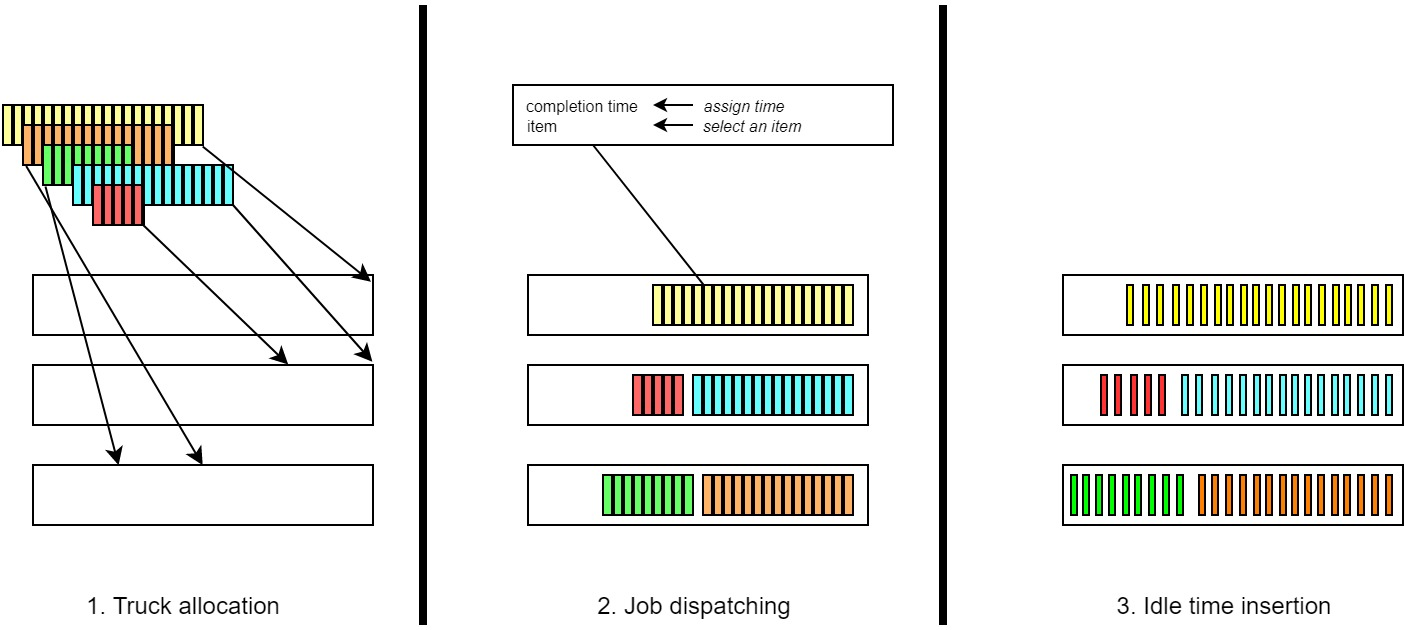
\includegraphics[width=1.0\linewidth]{algo.jpg}
\caption{Illustration of phases one to three of the algorithm.}
\end{figure}

\section{Truck allocation}

As said in Subsection \ref{subsec:truckallocation}, the goal of this phase is to distribute trucks among expedition ramps so that workers at each ramp work almost the same time and do nearly the same amount of work. This can be achieve by minimizing the makespan. By minimizing the makespan, we achieve good utilization of machines or in our case expedition ramps, which leads to balanced load on expedition ramps \cite{pinedo}. 

In many factories as well as in the automated warehouse, there are not many trucks scheduled for a single day (under 50). On top of that, truck allocation problem (\ref{subsec:truckallocation}) has very simple objective and constraints. This makes this problem a good example where CP or LP performs well. Even for it being a real-world problem, finding the optimal solution for this case is valuable since stochastic events like "need to reschedule a truck to different ramp" or "truck needs more or fewer items than it originally demanded" do not occur very often.

This problem was already formulated as assignment problem in Subsection \ref{subsec:truckallocation}, which can be solved using CP or LP method.

To improve the performance of these methods we need to select \textbf{upper bound} of the objective and variables. Upper bound is calculated using LPT heuristics mentioned in Chapter \ref{chap:Related work}. LPT heuristics can be also used as an alternative to CP or LP solution in cases where 

*In the CP approach, LPT heuristics can also be used for the ordering of variables. This way the algorithm redistributes trucks with lower load first, which can lead to uniformly distributed workload faster.

\section{Job dispatching}

At this phase, we need to determine which item will be handling what request and then assign a completion times (or start times) of processing of these requests.*

To be able to tell what is a feasible schedule and further describe this algorithm, we formulate this problem as a CSP. 

\subsubsection{CSP model}

\begin{itemize}
    \item Variables:\\
    \begin{equation}
        V = \{c_{0}, c_{1}, \ldots, x_{n}\}
    \end{equation}
    \begin{equation}
        W = \{r_0, \ldots, r_m\}
    \end{equation}
    \item Domains\\
    \begin{equation}
    c_{i} \in C_i = \{start, ..., end\}
    \end{equation}
    \begin{equation}
    r_{i} \in R
    \end{equation}
    \item Constraints
    \begin{equation}
    \begin{aligned}
    & noOverlap(c_i, r_i, c_j, r_j) &&\text{for } i=0,\ldots,n; j=0,\ldots,m\\
    & correctPosition(c_i, r_i, V, W) && \text{for } i=0,\ldots,n
    \end{aligned}
    \end{equation}
\end{itemize}

*correctPosition

Constraint $noOverlap$ prevents machines, conveyors and scanners to process more than one item at a time. Schedule is feasible if function $noOverlap$ is $True$ for every pair $i$,$j$.


The goal of this phase is to create a feasible schedule. To obtain it, a constructive heuristic method is proposed. This method assigns values to variables in a way that after assigning value to every variable, we get a feasible solution without a need to backtrack.

\begin{algorithm}[H]
\SetAlgoLined
\KwResult{A feasible schedule S}
  $items \leftarrow$ order $items$\;
 \For{$position \leftarrow 0$ \KwTo n}{
  $machines \leftarrow$ order machines\;
  \ForEach{$machine$ in $machines$}{
    $ramp \leftarrow$ select a ramp\;
    \ForEach{$i$ in $items$}{
    \If{$m_i = machine$}{
    \ForEach{$time$ in $C_i$}{
    \If{$S \cup \text{\{i, time, ramp\} is feasible}$}{
    Add \{i, time, ramp\} to solution S\;
    $items \leftarrow items \setminus \{i\}$\;
    $timeAssigned \leftarrow True$\;
    \textbf{goto} $mainLoopEnd$\;
}
}
}
}
}
[mainLoopEnd]\\
}
\caption{Heuristic construction}
\end{algorithm}

\subsubsection{Items ordering}
TBD

\subsubsection{Hybrid cyclic heuristics (Machines and ramp ordering)}
TBD

We need to select order at which a demanded item is expedited (see figure \ref{order})
\begin{figure}[h]
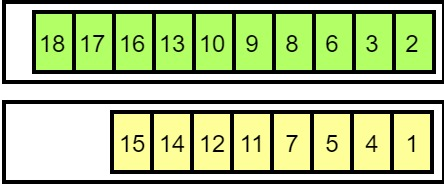
\includegraphics[width=0.8\linewidth]{order.jpg}
\caption{Diagram showing an ordering at which items are expedited.}
\label{order}
\end{figure}
\subsubsection{$C_i$ ordering}
TBD

\section{Idle time insertion}

The goal of this phase is to take advantage of the remaining working hours and spread the expedition through the whole day. Since order at which items are expedited is one of the requirements (subsection \ref{expedition}), inserting idle times is crucial for minimizing error in ordering due to delays caused by production handling.

Having a feasible schedule, we know how long it is, and we can tell approximately how much time we have until work hours end. We can take this time a distribute it among items as idle times. Unless there is only single expedition ramp, we cannot simply determine where or how big idle times we should insert; we have to run step 2 of the algorithm again after any insertion of idle times.

Each scheduled item is associated with an idle time, which follows after the completion time of the item. Other items cannot be scheduled after some item $i$ for its duration of idle time.

TBD

Idle times should be distributed uniformly to prevent buffer overflow too, but some items can benefit more from idle times (last item of its type).  Assign weights to each item (bigger weight, more likely to increase idle time). I propose distributing remaining time uniformly. Try to distribute remaining time, if the schedule is too long, try remaining time / 2, etc. until the remaining time is < something. After that, we can run simulated annealing to distribute the rest.

Simulated annealing applies the first move that improves or does not change a score. The set of moves that is proposed is *... and order at which moves are consider is based on weight of an item and length of already assigned idle time. 

*formula

\section{Re-ordering}
*Above is also local search, maybe merge?.

Another improvement is using tabu search which swaps order number of two items. Some objectives are not easily minimized using some heuristics in step 2 like for example weighted penalty for scheduling two jobs right after each other on a single machine because it can lead to stopping a production

\chapter{Implementation}
\section{Simulation environment}
\section{Scheduler module}
\chapter{Evaluation}
\label{ch:Evaluation}
\section{Performance}
\section{Scenarios}
\section{Comparison}
\subsection{Comparison of plan and behavior in simulation}
Comparing different version (LS, no LS, heuristic 1, heuristic 2, ...) of algorithm too.
\subsection{Effect of objectives?}
Mainly significance of idle times (at scanner or machines)
\chapter{Conclusion}

Lorep ipsum \cite{doe}

\begin{thebibliography}{1}
\bibitem{warehousepic} GILGEN LOGISTICS AG. \emph{Automated high-bay warehouse} [online]. 4 December 2016. Available from: https://commons.wikimedia.org/wiki/File:Automatisches\_Hochregallager\_mit\_Regalbediengeräten.jpg
\bibitem{doe} J. Doe. \emph{Book on foobar.} Publisher X,
 2300.
 \bibitem{gram1969} R.L. Graham (1969) \emph{Bounds on Multiprocessing Timing Anomalies}, SIAM
Journal of Applied Mathematics, Vol. 17, pp. 263–269
\bibitem{complexity} A.H.G. Rinnooy Kan (1976) \emph{Machine Scheduling Problems: Classification,
Complexity and Computations}, Nijhoff, The Hague (as cited in \cite{pinedo})


\end{thebibliography}

***
The order at which trucks arrive at the expedition ramp is determined by priority of a truck. A truck with higher priority is scheduled before a truck with lower priority on the same expedition ramp. If a truck is delayed, it affects trucks scheduled after it and it creates cascading effect, where all trucks behind the first delayed one are delayed if reserve time between them is not big enough. 


\label{overlap}
\begin{algorithm}[H]
\SetAlgoLined
\SetKwInOut{Input}{input}\SetKwInOut{Output}{output}
\Input{$c_i$ - completion time of an item $i$, $c_j$ - completion time of an item $j$, $r_i$ ramp to which item $i$ is assigned, $r_j$ ramp to which an item $j$ is assigned\\}
\Output{$1$ - Process of unloading items $i$ and $j$ does not overlap, $0$ - Process of unloading items $i$ and $j$ overlaps either at stacker crane, scanner or a conveyor}

$s_i = c_i - s\;$\\
$s_j = c_j - s\;$\\
$scc_i = s_i - t_{r_i}\;$\\
$scc_j = s_j - t_{r_j}\;$\\

$scs_i = scc_i - p_i\;$\\
$scs_j = scc_j - p_j\;$

\If{$m_i = m_j$}{
    \If{$scc_i > scs_j \land scc_j > scs_i$}{
        return $0\;$ \tcc{Processing of an items $i$ and $j$ is overlapping at stacker crane $m_i$}
    }
}

\If{$r_i = r_j$}{
    \If{$c_i  + \theta_i > s_j \land c_j + \theta_j > s_i$}{
        return $0\;$ \tcc{Processing of an items $i$ and $j$ is overlapping at expedition ramp $r_i$}
    }
}

return $1\;$
 \caption{Constraint - noOverlap}
\end{algorithm}
\end{document}

